%UCE-1: Modifica funzioni di sistema

Nel proseguo dei paragrafi relativi ai casi d'uso \emph{UCE}, il nome dell'attore \emph{Environment Developer} verrà abbreviato con la sigla \emph{ED}.

\begin{figure}
\centering
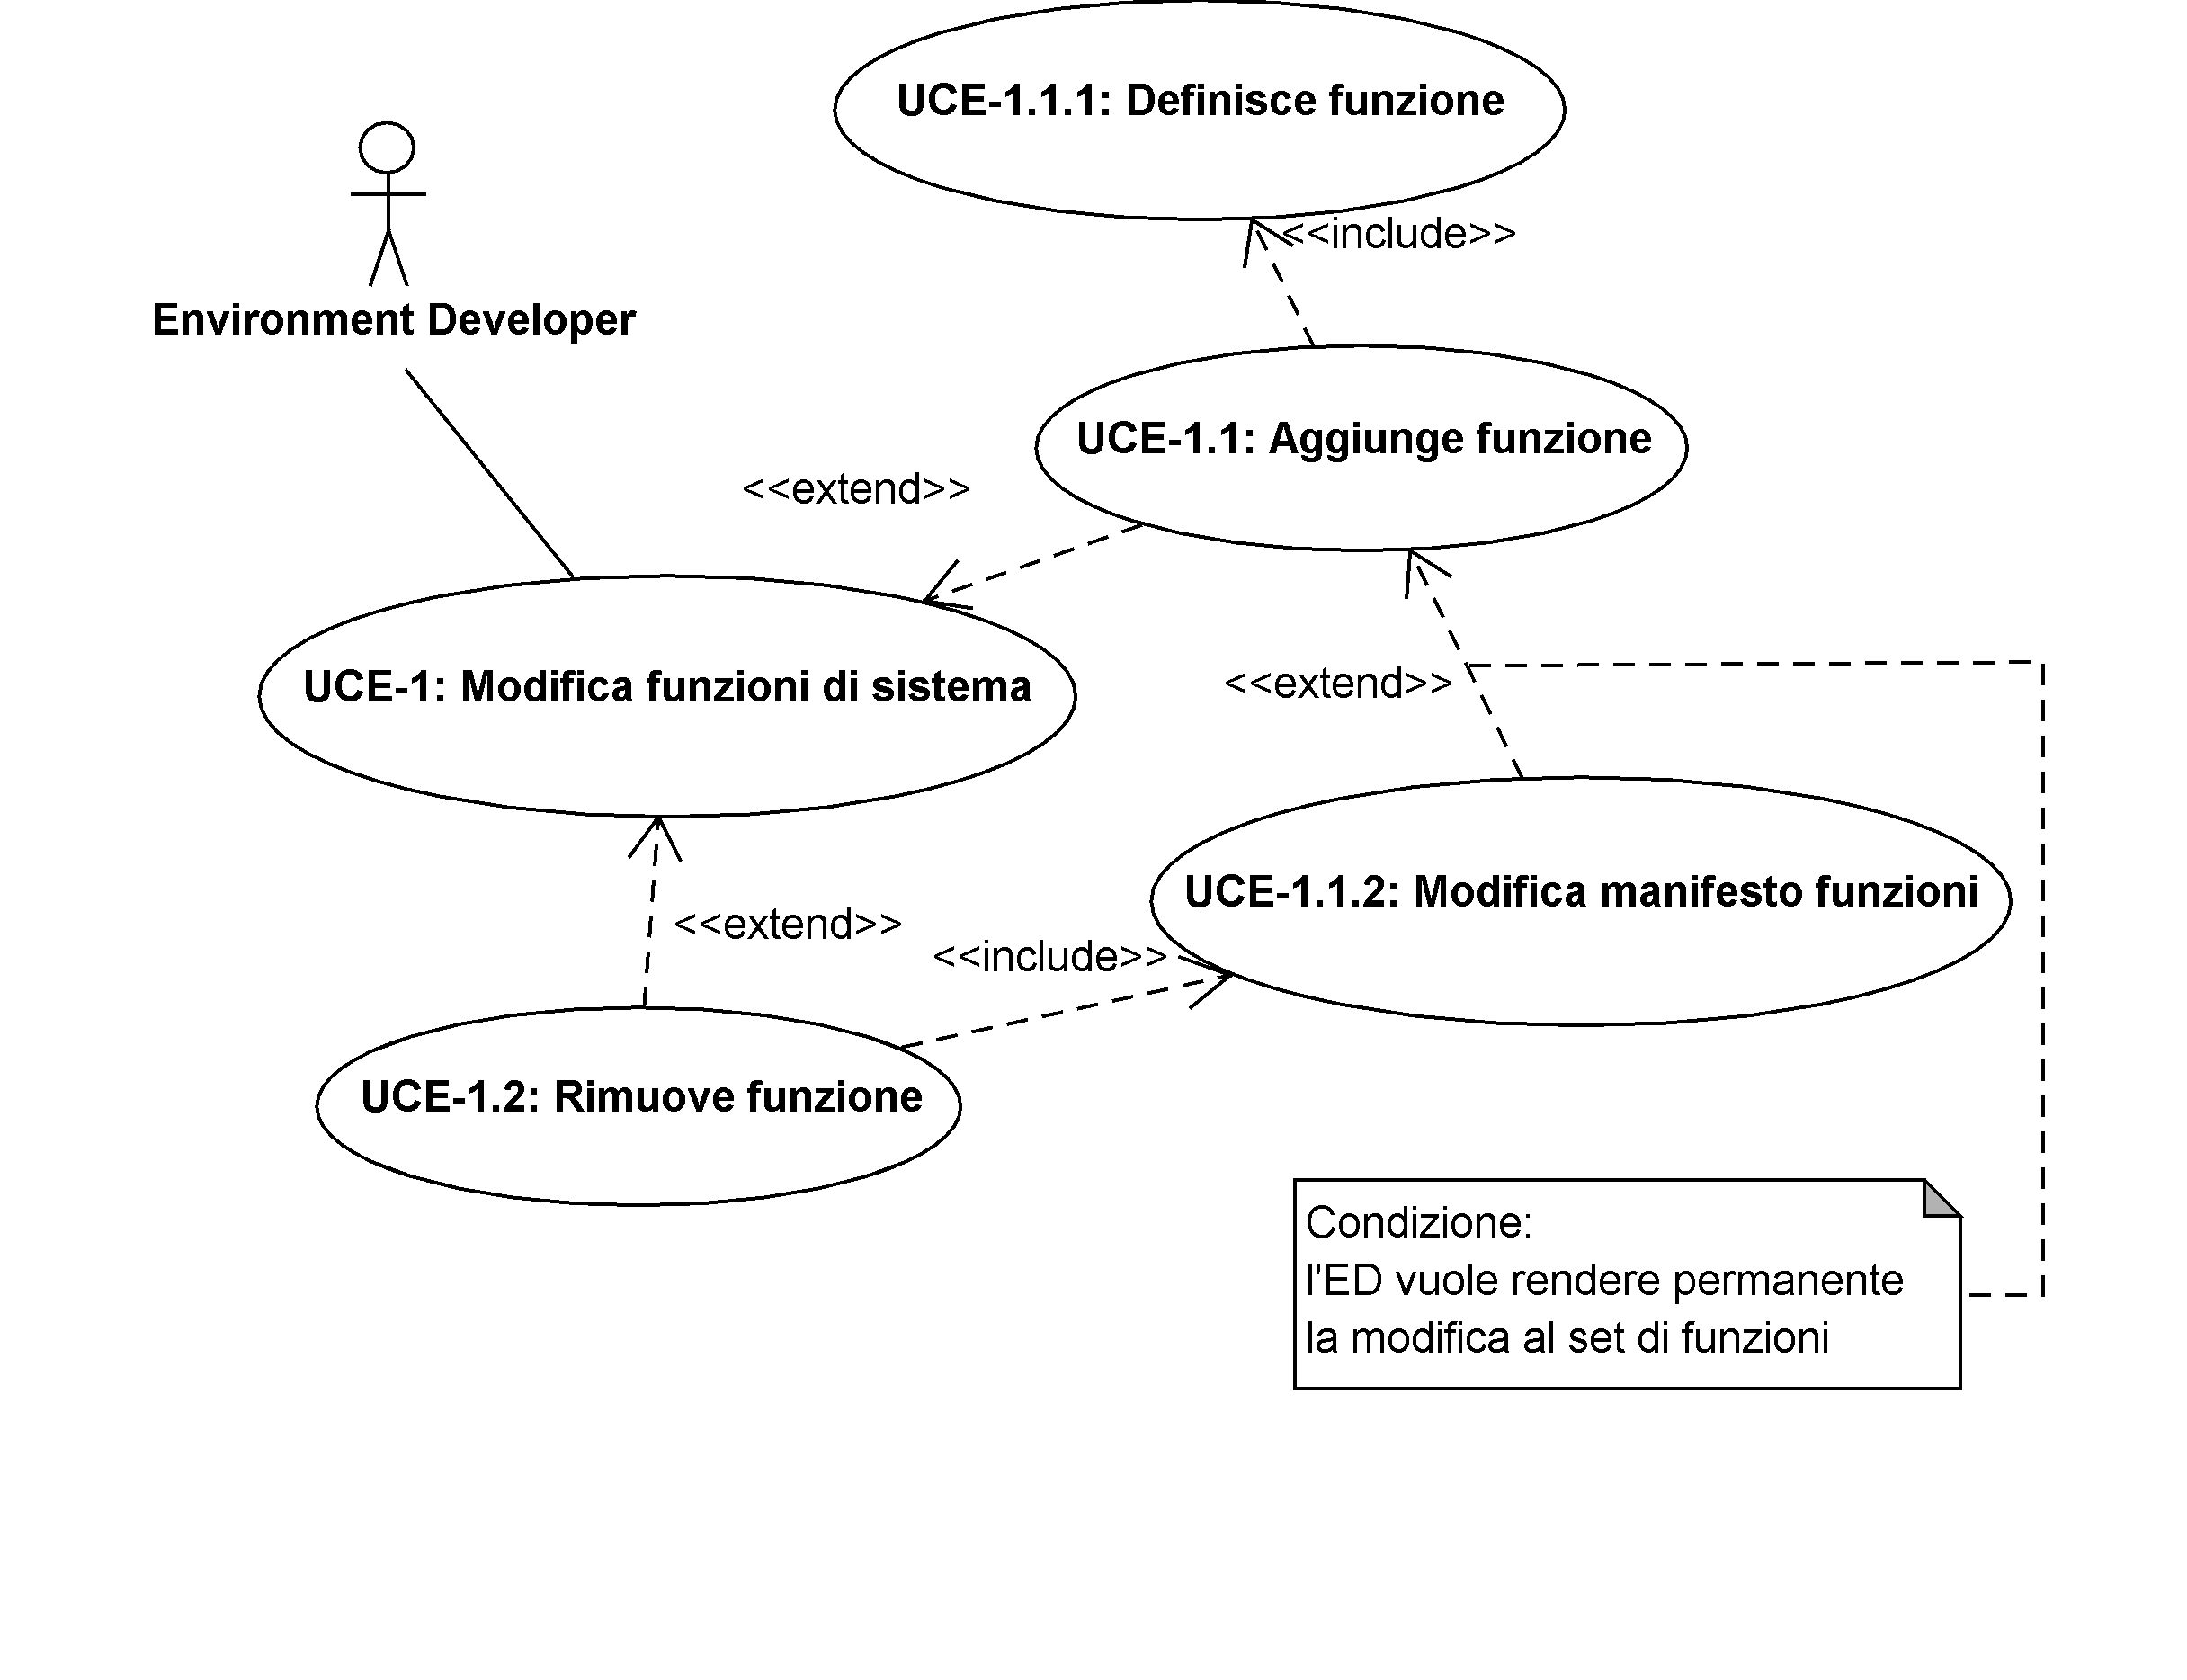
\includegraphics[width=1.1\textwidth]{Immagini/Capitolo2/UseCases/UCE-1.png}
\caption{Diagramma dei casi d'uso UCE-1}\label{fig:uc-uce-1}
\end{figure}


\begin{itemize}
	\item \textbf{Attori:} Environment Developer (\emph{ED})
	\item \textbf{Scopo e descrizione:} l'ED deve essere in grado di modificare il set di funzioni di sistema incluse nel software
	\item \textbf{Pre-condizioni:} il software fornisce meccanismi per estendere il set di funzioni di sistema
	\item \textbf{Post-condizioni:} il set di funzioni di sistema risulta modificato
	\item \textbf{Flusso principale degli eventi:}
		\begin{enumerate}
			\item l'ED esegue una modifica al set di funzioni di sistema.
			\begin{itemize}
				\item l'ED può rimuovere la definizione di una funzione esistente (si veda caso d'uso \emph{UCE-1.2})
				\item l'ED può aggiungere una nuova definizione di funzione di sistema (si veda caso d'uso \emph{UCE-1.1}).
			\end{itemize}
			\item il sistema carica il set modificato di funzioni sistema.
		\end{enumerate}
\end{itemize}


\paragraph{UCE-1.1: Aggiunge funzione}

La descrizione comprende quella del caso d'uso \emph{UCE-1.1.1}

\begin{itemize}
	\item \textbf{Attori:} ED
	\item \textbf{Scopo e descrizione:} un ED deve essere in grado di aggiungere una nuova funzione al set di funzioni di sistema.
	\item \textbf{Pre-condizioni:} il sistema è stato configurato correttamente. Il sistema non è attivo
	\item \textbf{Post-condizioni:} il sistema è attivo e una nuova funzione è disponibile nel set di funzioni di sistema
	\item \textbf{Flusso principale degli eventi:}
		\begin{enumerate}
			\item l'ED definisce il corpo di una nuova funzione di sistema (\emph{UCE-1.1.1})
			\item l'ED definisce la firma di una nuova funzione di sistema
				\begin{itemize}
					\item l'ED specifica un nome di funzione
					\item l'ED specifica un numero di parametri accettati (minimi, massimi, esatti)
					\item l'ED specifica il tipo dei parametri accettati
					\item l'ED specifica il tipo dei risultati
				\end{itemize}
			\item l'ED avvia il software
			\item l'ED richiede al software il caricamento della nuova funzione
				\begin{itemize}
					\item l'ED indica il file contenente il corpo della funzione
					\item l'ED indica la posizione della firma della funzione
				\end{itemize}
			\item la richiesta è valutata dal sistema
			\item la nuova definizione viene resa disponibile
		\end{enumerate}
	\item \textbf{Flusso alternativo \#1:}
		\begin{enumerate}
			\setcounter{enumi}{4}
			\item se l'ED ha specificato un nome di funzione già utilizzato, il sistema ignora la nuova definizione, notificando l'errore
		\end{enumerate}

	\item \textbf{Flusso alternativo \#2:}
		\begin{enumerate}
			\setcounter{enumi}{1}
			\item l'ED definisce la firma della nuova funzione indicando solo il nome e il tipo dei risultati della funzione
			\item \emph{analogo al punto 3 del flusso principale}
			\item \emph{analogo al punto 4 del flusso principale}
			\item \emph{analogo al punto 5 del flusso principale}						
			\item la firma viene integrata automaticamente dal sistema in modo che la funzione accetti un numero ed un tipo arbitrario di valori
			\item lo scenario prosegue con il punto 6 del flusso principale
		\end{enumerate}

	
\end{itemize}


\subparagraph{UCE-1.1.2: Modifica manifesto funzioni} % nome del caso d'uso SottoGruppo

\begin{itemize}
	\item \textbf{Attori:} ED
	\item \textbf{Scopo e descrizione:} ED deve essere in grado di apportare una modifica permanente al set di funzioni di sistema modificando un registro contenente l'elenco di funzioni di sistema
	\item \textbf{Pre-condizioni:} l'ED vuole rendere permanente l'aggiunta o la rimozione di una funzione di sistema. Il software non è attivo.
	\item \textbf{Post-condizioni:} il software è attivo, la modifica apportata al registro viene evidenziata nel set di funzioni di sistema disponibili
	\item \textbf{Flusso principale degli eventi:}
		\begin{enumerate}
			\item l'ED modifica il registro contenente l'elenco delle funzioni di sistema
				\begin{itemize}
					\item l'ED può aggiungere una nuova funzione all'elenco specificando il file contenente il corpo e la posizione della firma della funzione
					\item l'ED può rimuovere una funzione eliminandone le informazioni dall'elenco
				\end{itemize}
			\item l'ED salva le modifiche al registro
			\item l'ED avvia il sistema
			\item le modifiche vengono valutate dal sistema
			\item il set di funzioni disponibili viene modificato
			\item l'inizializzazione del software prosegue
		\end{enumerate}
	\item \textbf{Flusso alternativo:} 
		\begin{enumerate}
			\setcounter{enumi}{4}
			\item se l'ED ha apportato modifiche non valide al registro delle funzioni di sistema, il software notifica l'errore
			\item l'inizializzazione del software viene arrestata
		\end{enumerate}
\end{itemize}


\paragraph{UCE-1.2: Rimuove funzione}

\begin{itemize}
	\item \textbf{Attori:} ED
	\item \textbf{Scopo e descrizione:} ED deve essere in grado di rimuovere una funzione di sistema da quelle disponibili.
	\item \textbf{Pre-condizioni:} il software è configurato correttamente, il software non è attivo.
	\item \textbf{Post-condizioni:} Il software è attivo, la funzione di sistema non è presente fra quelle disponibili
	\item \textbf{Flusso principale degli eventi:}
		\begin{enumerate}
			\item l'ED modifica il manifesto delle funzioni di sistema rimuovendo le informazioni riguardanti la funzione (si guardi caso il d'uso \emph{UCE-1.1.2})
		\end{enumerate}
\end{itemize}

